\section{YouTube接続設定 \index{youtube@YouTube}}
YouTubeとの接続には、\lastfm というサービスと、そこへ再生履歴を反映するための「Scrobble」という機能をもつアプリの2つが必要です。
    \begin{figure}[htbp]
        \centering
        \fbox{
            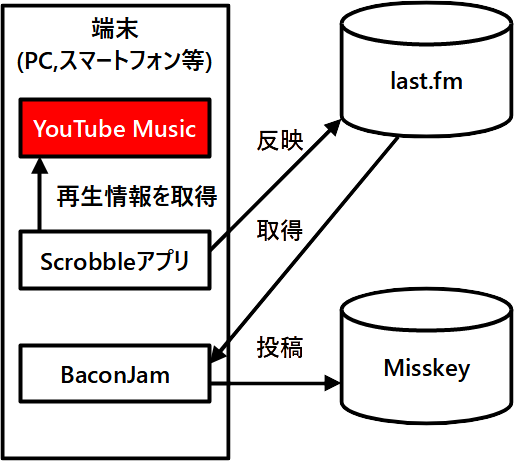
\includegraphics[width=10cm]{./pictures/lastfm1.png}
        }
        \caption{YouTubeとの連携イメージ図}
        \label{img:lastfm1}
    \end{figure}

    \newpage
    \subsection{\lastfm 側の設定}
        \begin{enumerate}
            \item アカウントをお持ちでない場合は、\href{https://www.last.fm}{last.fm}にアクセスし、アカウントを作成してください。
            \item \href{https://www.last.fm/api}{Last.fm Music Discovery API}にアクセスし、\href{https://www.last.fm/api/account/create}{Get an API account}を押下してください。
                \begin{figure}[htbp]
                    \centering
                    \fbox{
                        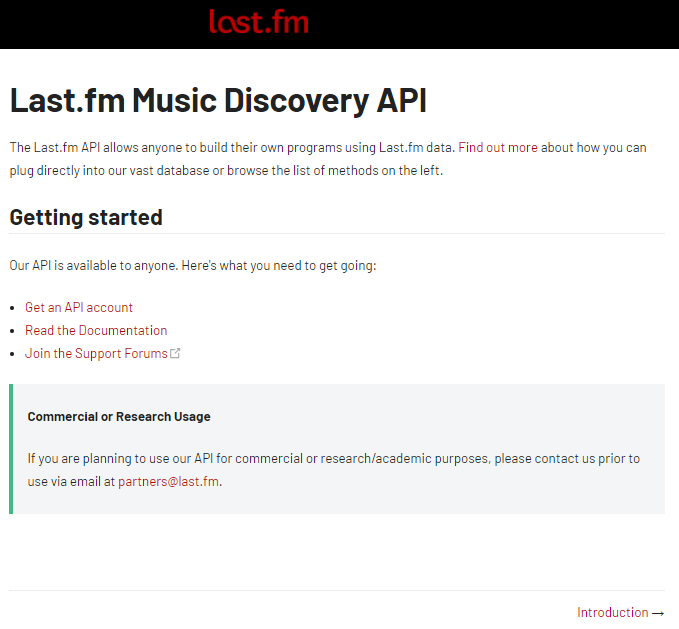
\includegraphics[width=8cm]{./pictures/lastfm2.png}
                    }
                    \caption{Last.fm Music Discovery API}
                    \label{img:lastfm2}
                \end{figure}

            \newpage
            \item APIアカウント作成ページが表示されるので、以下を参考に値を設定して\ttbox{SUBMIT}を押下してください。
                \begin{figure}[htbp]
                    \centering
                    \fbox{
                        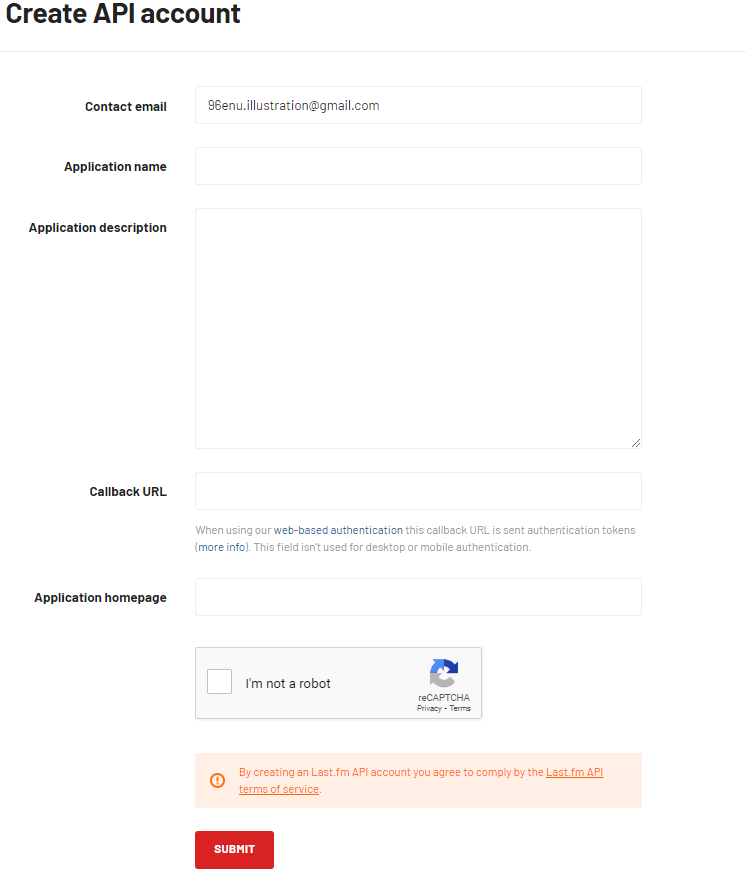
\includegraphics[width=8cm]{./pictures/lastfm3.png}
                    }
                    \caption{APIアカウント作成ページ}
                    \label{img:lastfm3}
                \end{figure}
                \begin{itemize}
                    \item \texttt{Contact email}…last.fmアカウント作成時に使用したメールアドレスが初期設定されているので、そのままで構いません。
                    \item \texttt{Application name}…なんらかの値を設定してください\footnote{自由な値で構いませんが、\bj 用のappであることが分かるような名前の設定を推奨します。}。
                    \item \texttt{Application description}…空欄で構いません。
                    \item \texttt{Callback URL}…空欄で構いません。
                    \item \texttt{Application homepage}…空欄で構いません。
                \end{itemize}

            \newpage
            \item \imageref{img:lastfm4}のようなページに切り替わったら、APIアカウントが正しく作成されています。このページの\texttt{API key}の値を控えてください\footnote{値を忘れてしまった場合は、\href{https://www.last.fm/api/accounts}{APIアプリケーション一覧ページ}で再度確認してください。}。
                \begin{figure}[htbp]
                    \centering
                    \fbox{
                        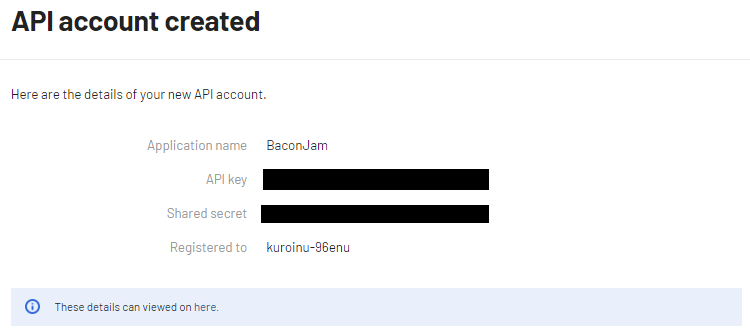
\includegraphics[width=8cm]{./pictures/lastfm4.png}
                    }
                    \caption{APIアカウント作成完了ページ}
                    \label{img:lastfm4}
                \end{figure}
        \end{enumerate}

    \newpage
    \subsection{連携用アプリの設定}
        ここでは、\href{https://play.google.com/store/apps/details?id=com.arn.scrobble&hl=ja&gl=US}{Pano Scrobbler}を使用した場合について解説します。
        \begin{enumerate}
            \item スマートフォンに\href{https://play.google.com/store/apps/details?id=com.arn.scrobble&hl=ja&gl=US}{Pano Scrobbler}をインストールしてください。
            \item Pano Scrobblerを起動して\ttbox{Last.fm}を押下してログインし、\ttbox{YES, ALLOW ACCESS}を押下してください。
                \begin{figure}[htbp]
                    \begin{minipage}[b]{0.45\linewidth}
                        \centering
                        \fbox{
                            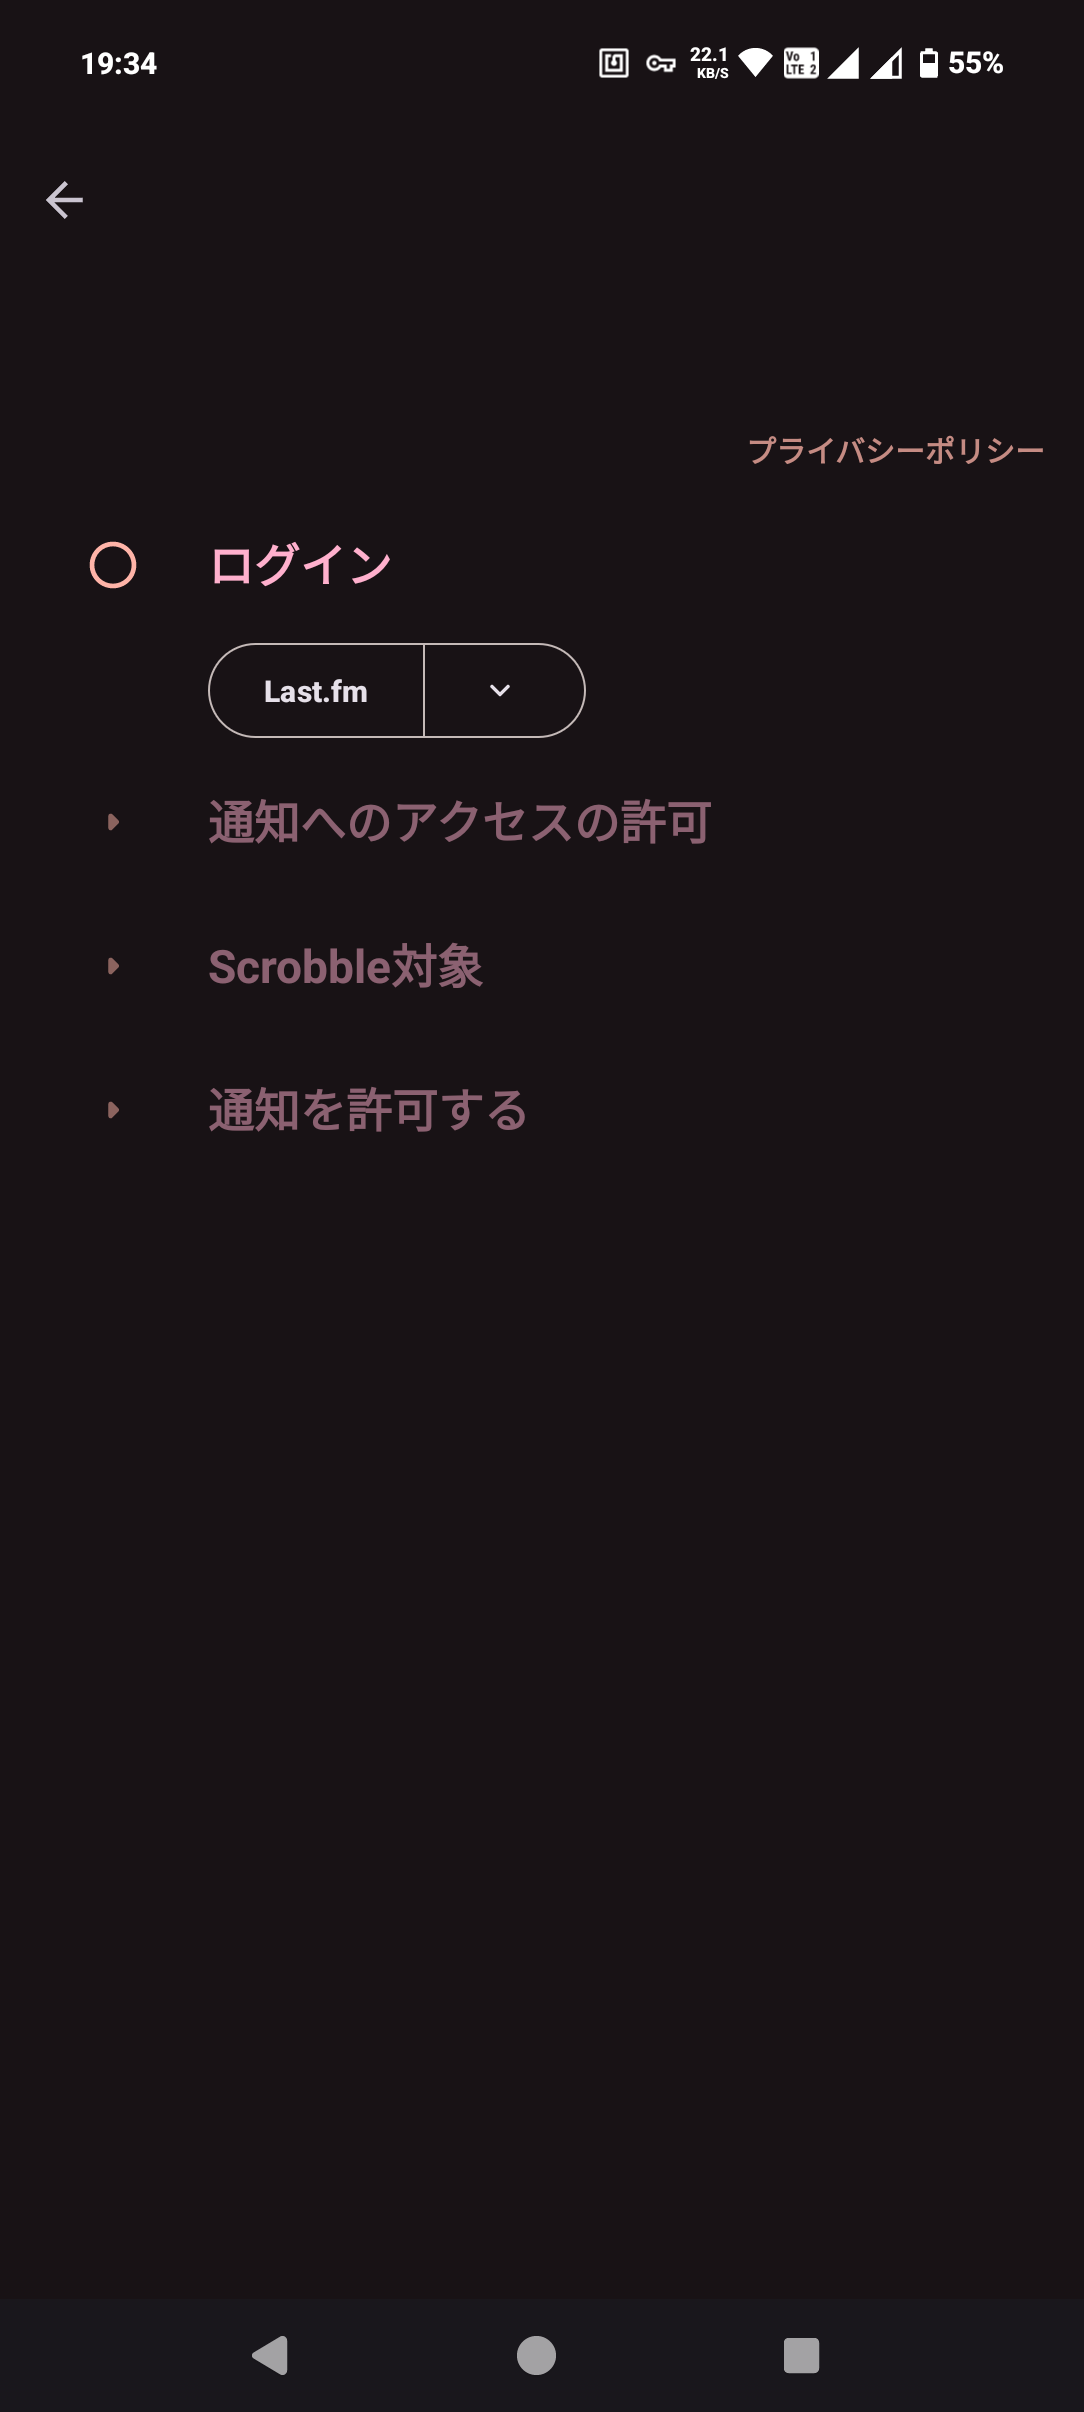
\includegraphics[width=5cm]{./pictures/lastfm5.png}
                        }
                        \label{img:lastfm5}
                    \end{minipage}
                    \begin{minipage}[b]{0.45\linewidth}
                        \centering
                        \fbox{
                            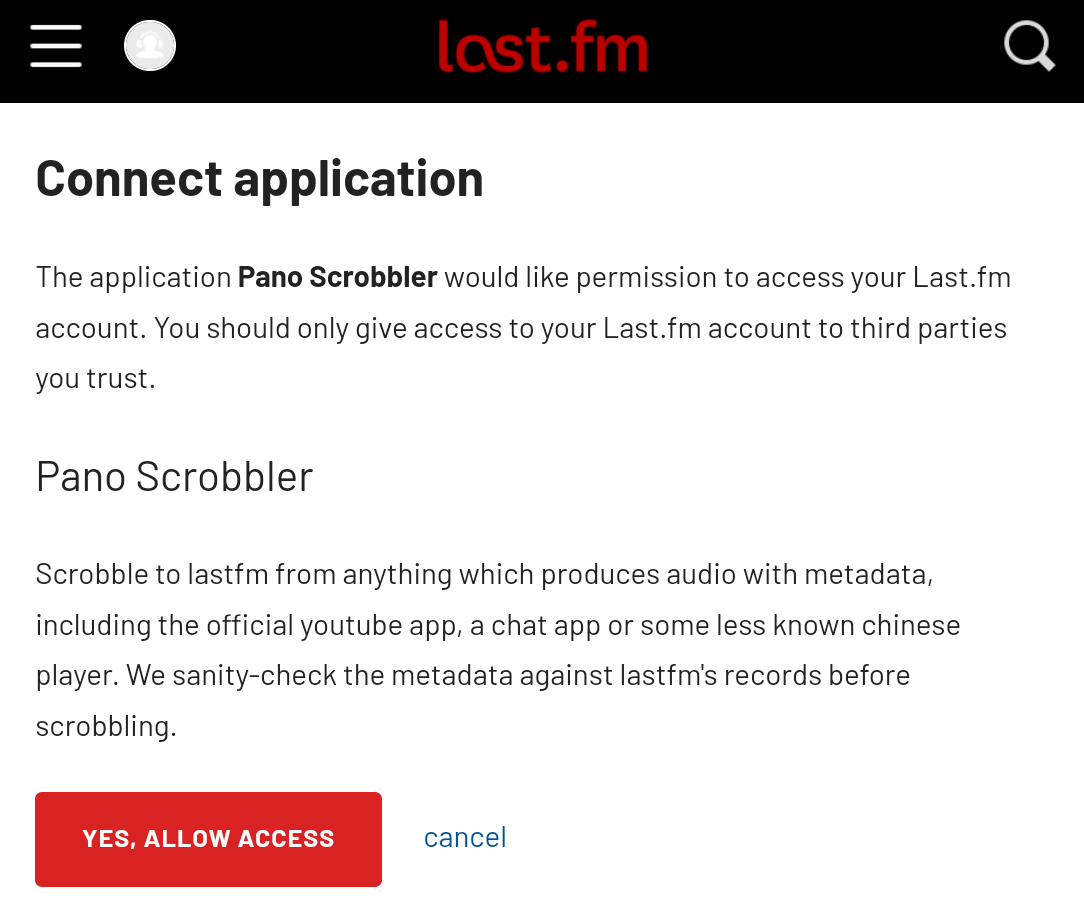
\includegraphics[width=5cm]{./pictures/lastfm6.png}
                        }
                        \label{img:lastfm6}
                    \end{minipage}
                    \caption*{ログイン}
                \end{figure}

            \newpage
            \item 通知へのアクセスを許可してください。
            \item Scrobble対象の\ttbox{開く}を押下して、YouTube Musicのみにチェックが入った状態にしてください。
                \begin{figure}[htbp]
                    \begin{minipage}[b]{0.45\linewidth}
                        \centering
                        \fbox{
                            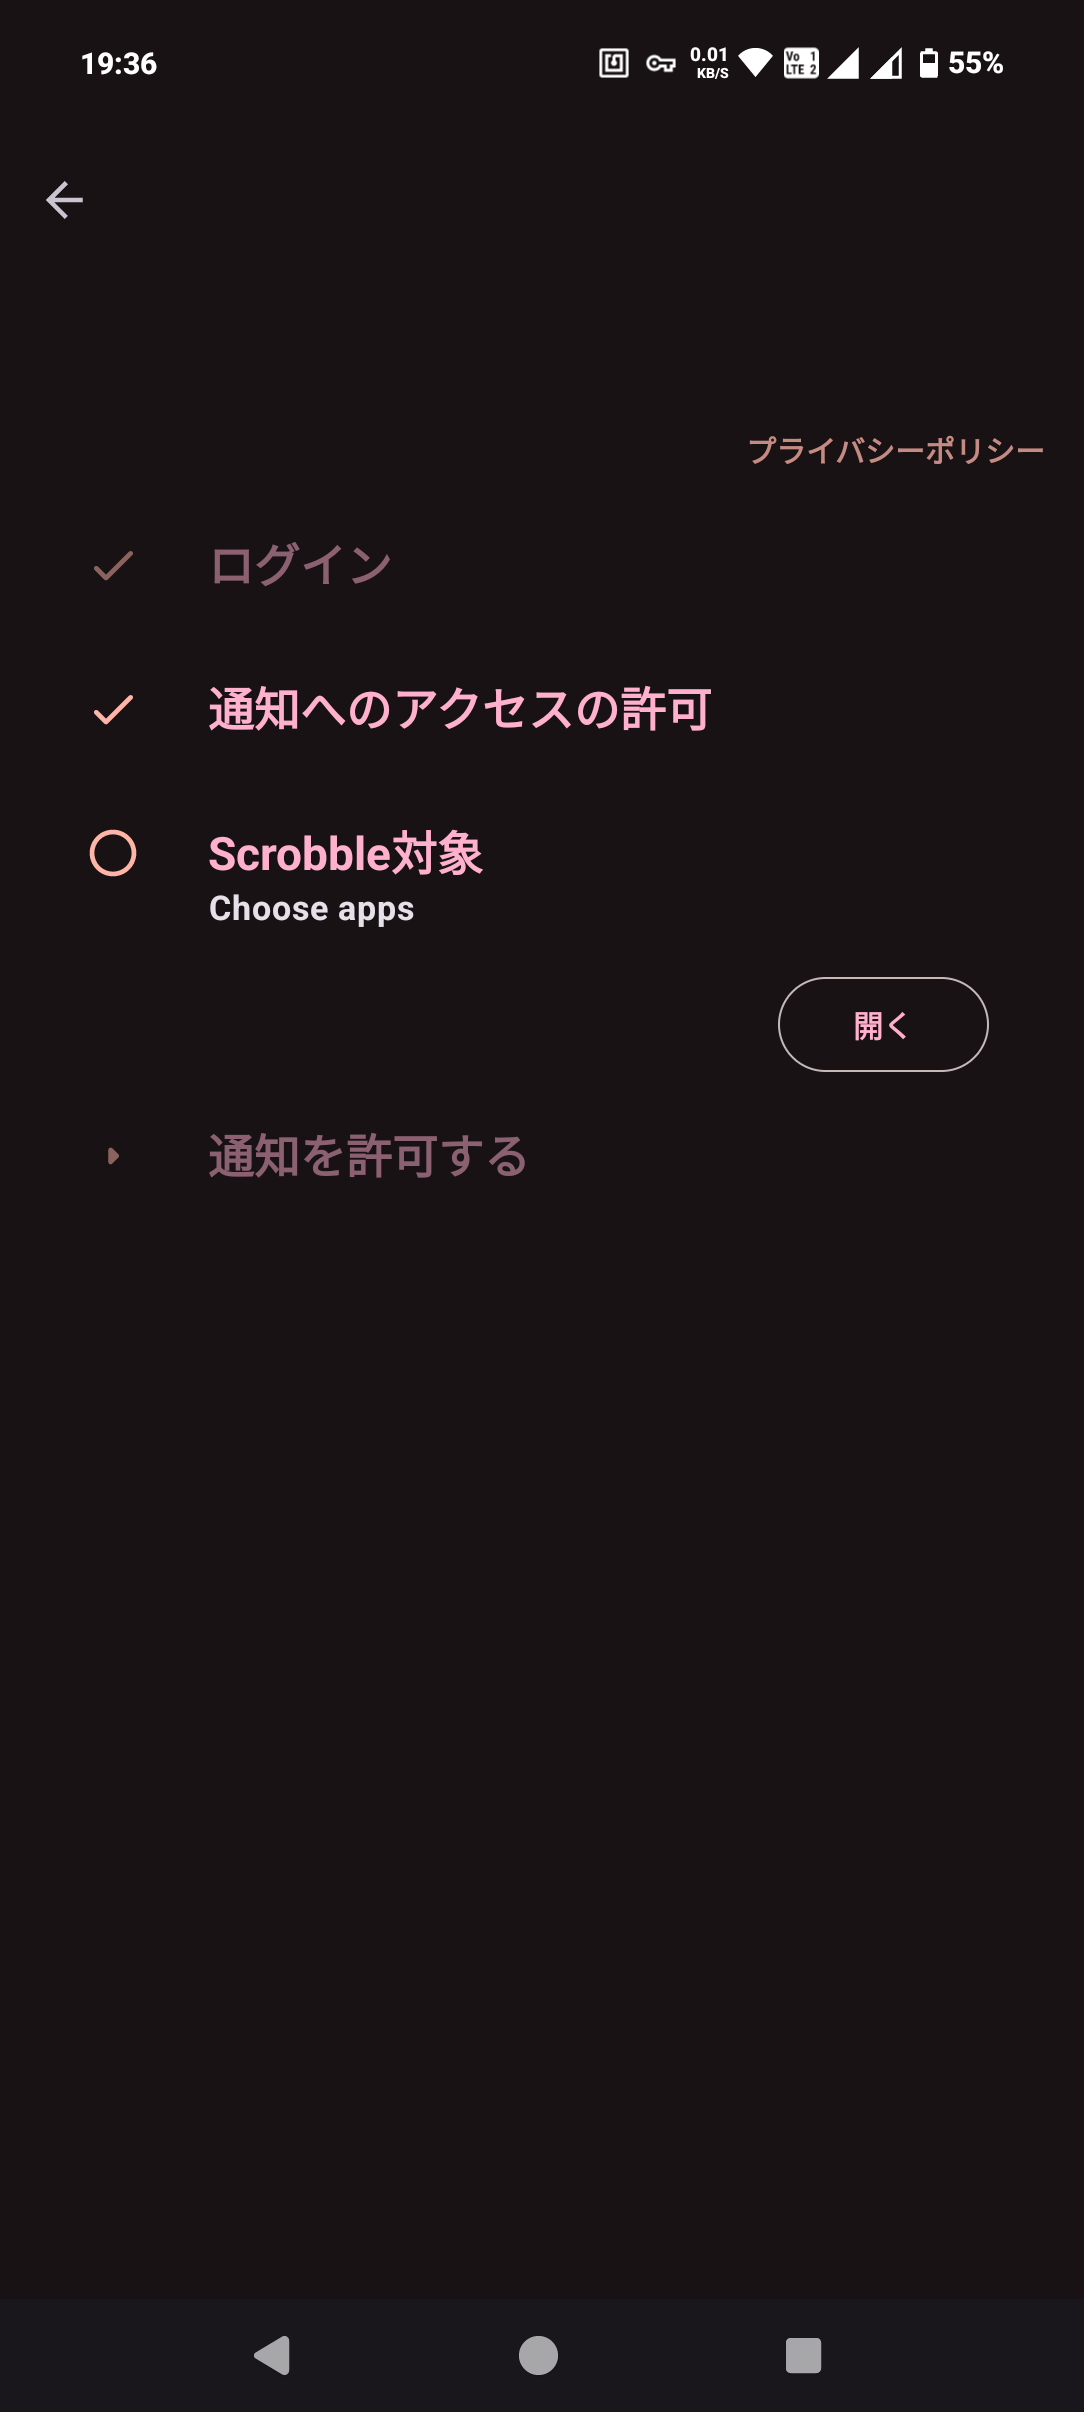
\includegraphics[width=5cm]{./pictures/lastfm8.png}
                        }
                        \label{img:lastfm8}
                    \end{minipage}
                    \begin{minipage}[b]{0.45\linewidth}
                        \centering
                        \fbox{
                            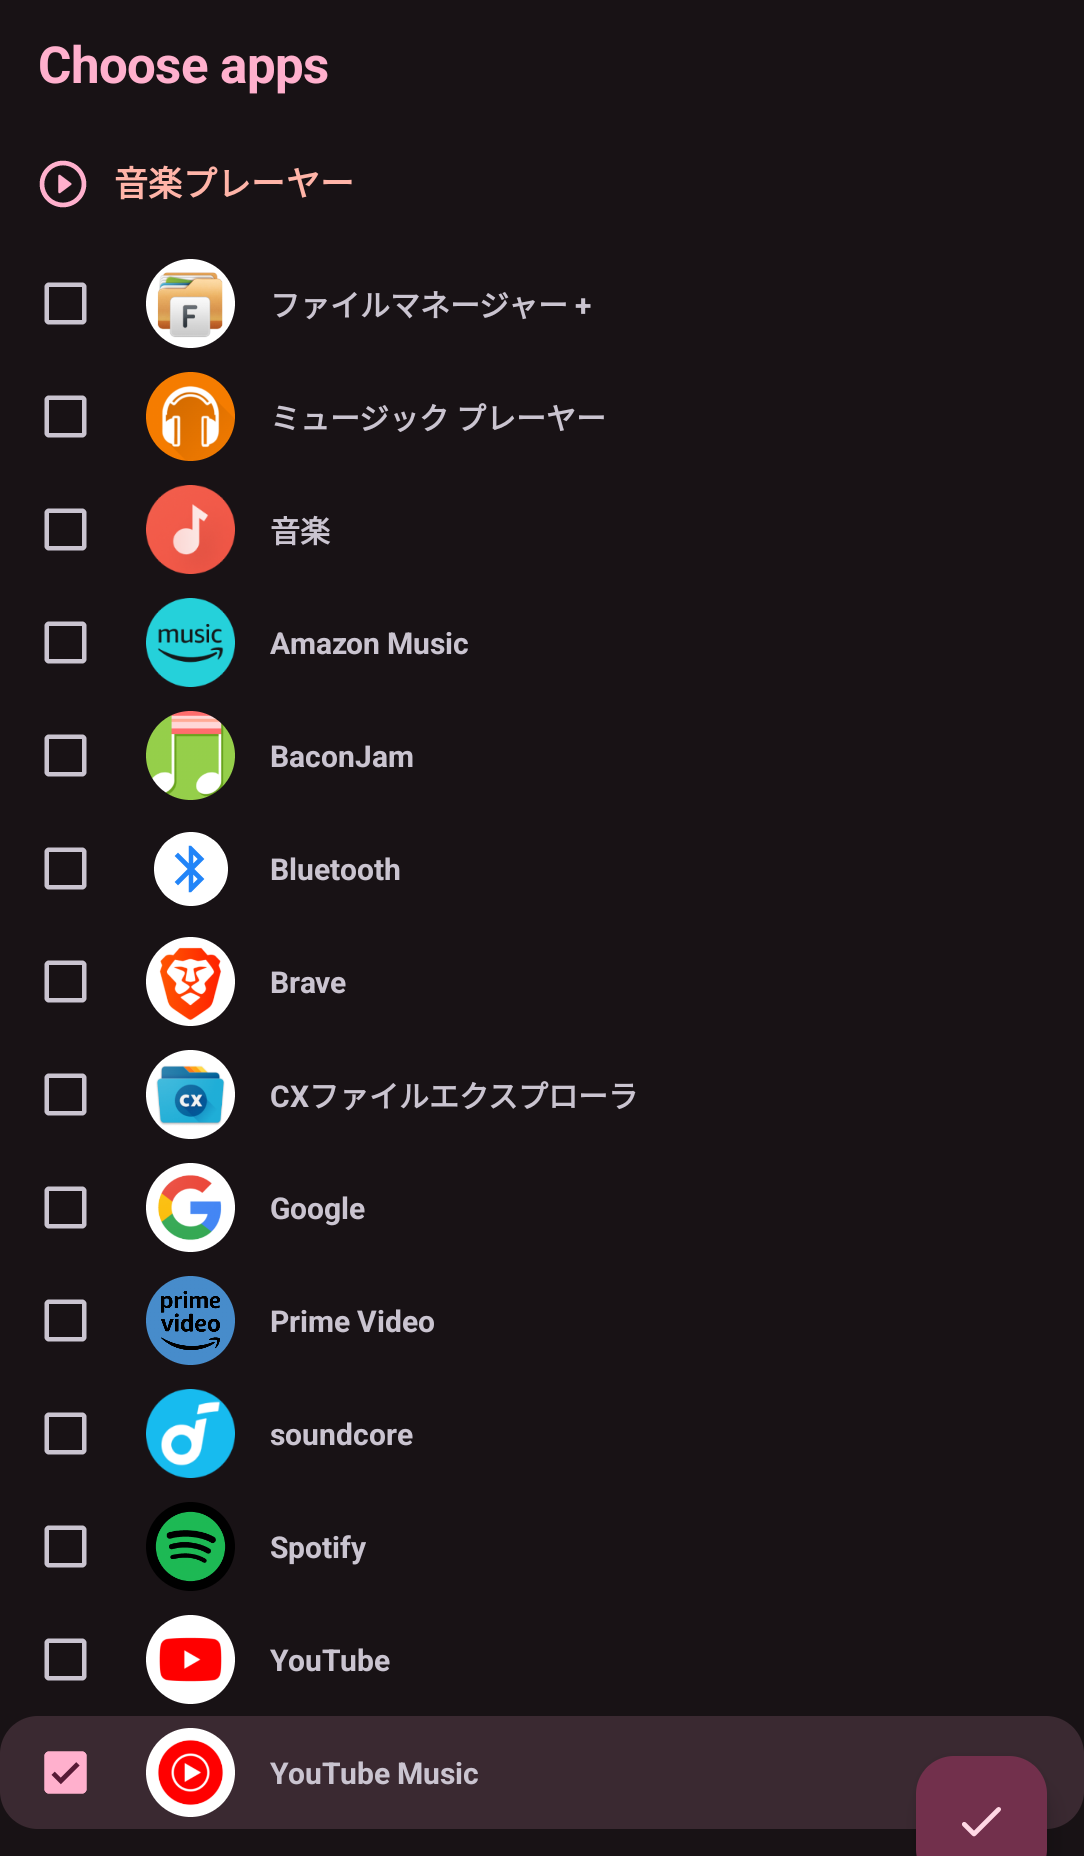
\includegraphics[width=5cm]{./pictures/lastfm9.png}
                        }
                        \label{img:lastfm9}
                    \end{minipage}
                    \caption*{対象アプリ選択}
                \end{figure}
            \item 通知を許可してください。

            \newpage
            \item アプリの設定を開き、「Scrobbleの遅延」の「分」を最小の30秒に設定したら、Pano Scrobblerの設定は完了です。
                \begin{figure}[htbp]
                    \centering
                    \fbox{
                        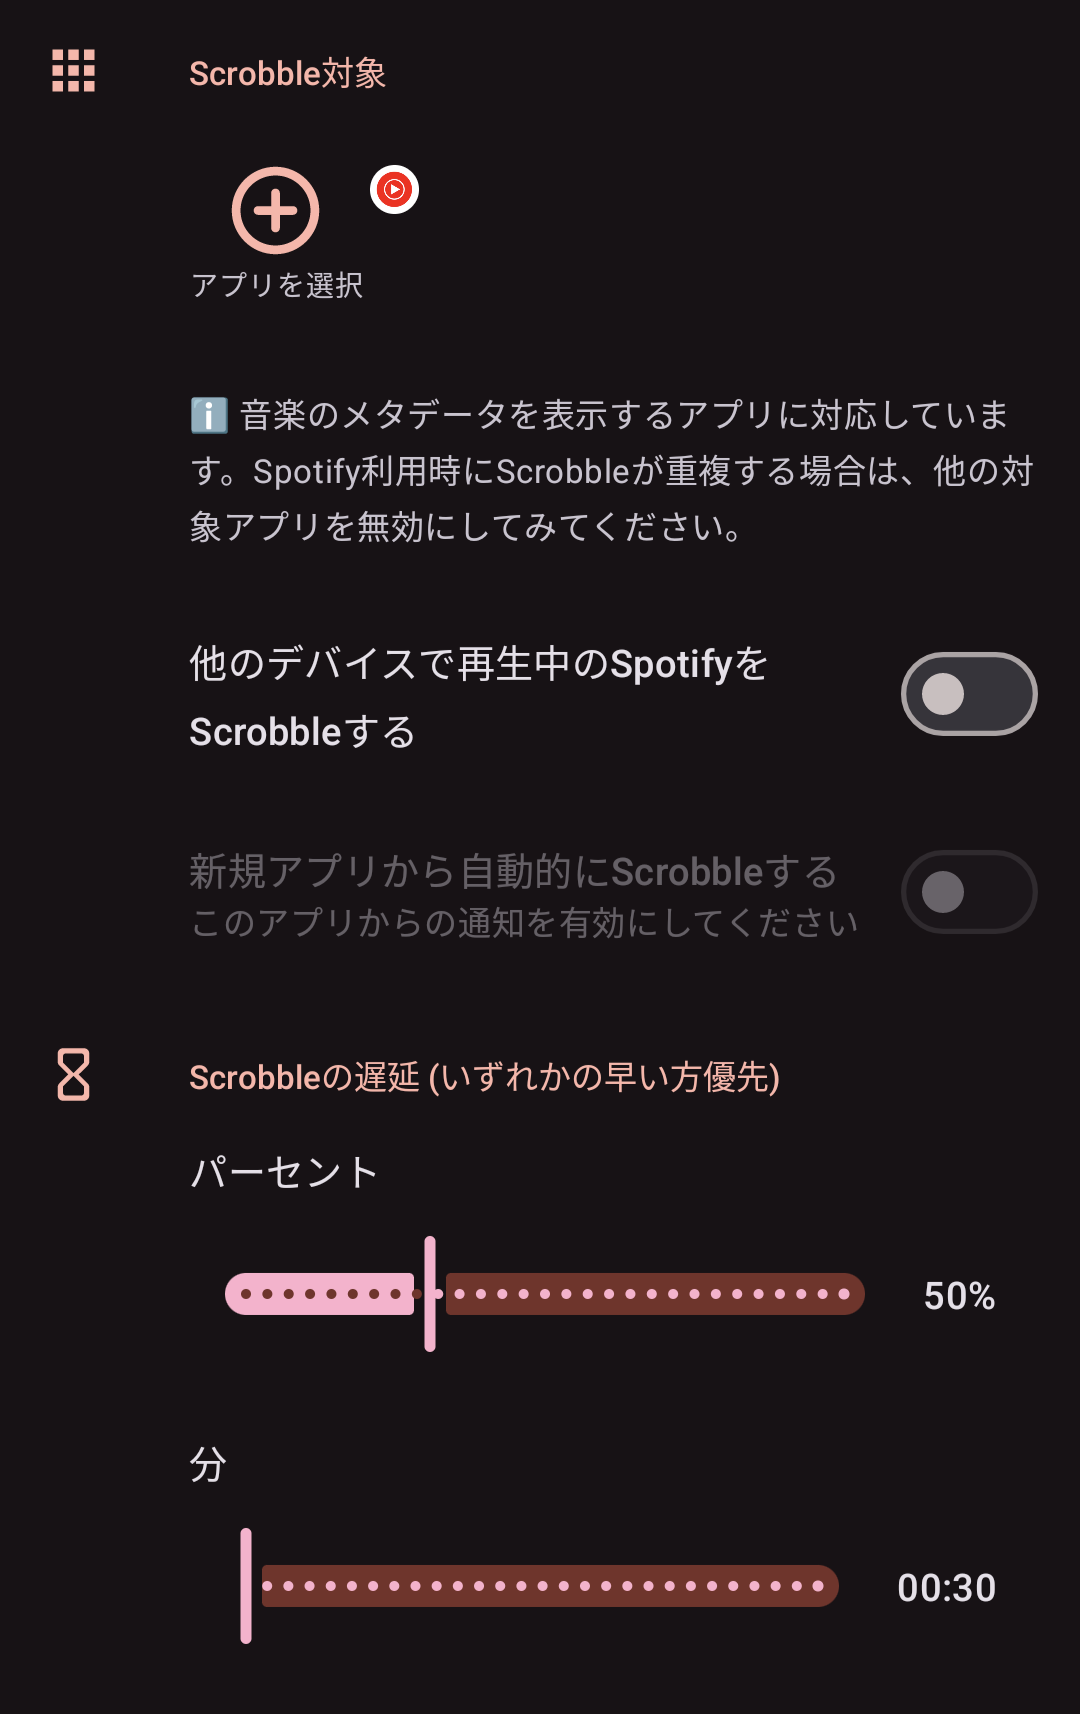
\includegraphics[width=6cm]{./pictures/lastfm10.png}
                    }
                    \caption{Scrobbleの遅延}
                    \label{img:lastfm10}
                \end{figure}
        \end{enumerate}

    \newpage
    \subsection{\bj 側の設定}
        \begin{enumerate}
            \item 設定画面の\ttbox{YouTube接続設定(プレビュー版)}を押下して、設定項目を展開してください。
                \begin{figure}[htbp]
                    \begin{minipage}[b]{0.45\linewidth}
                        \centering
                        \fbox{
                            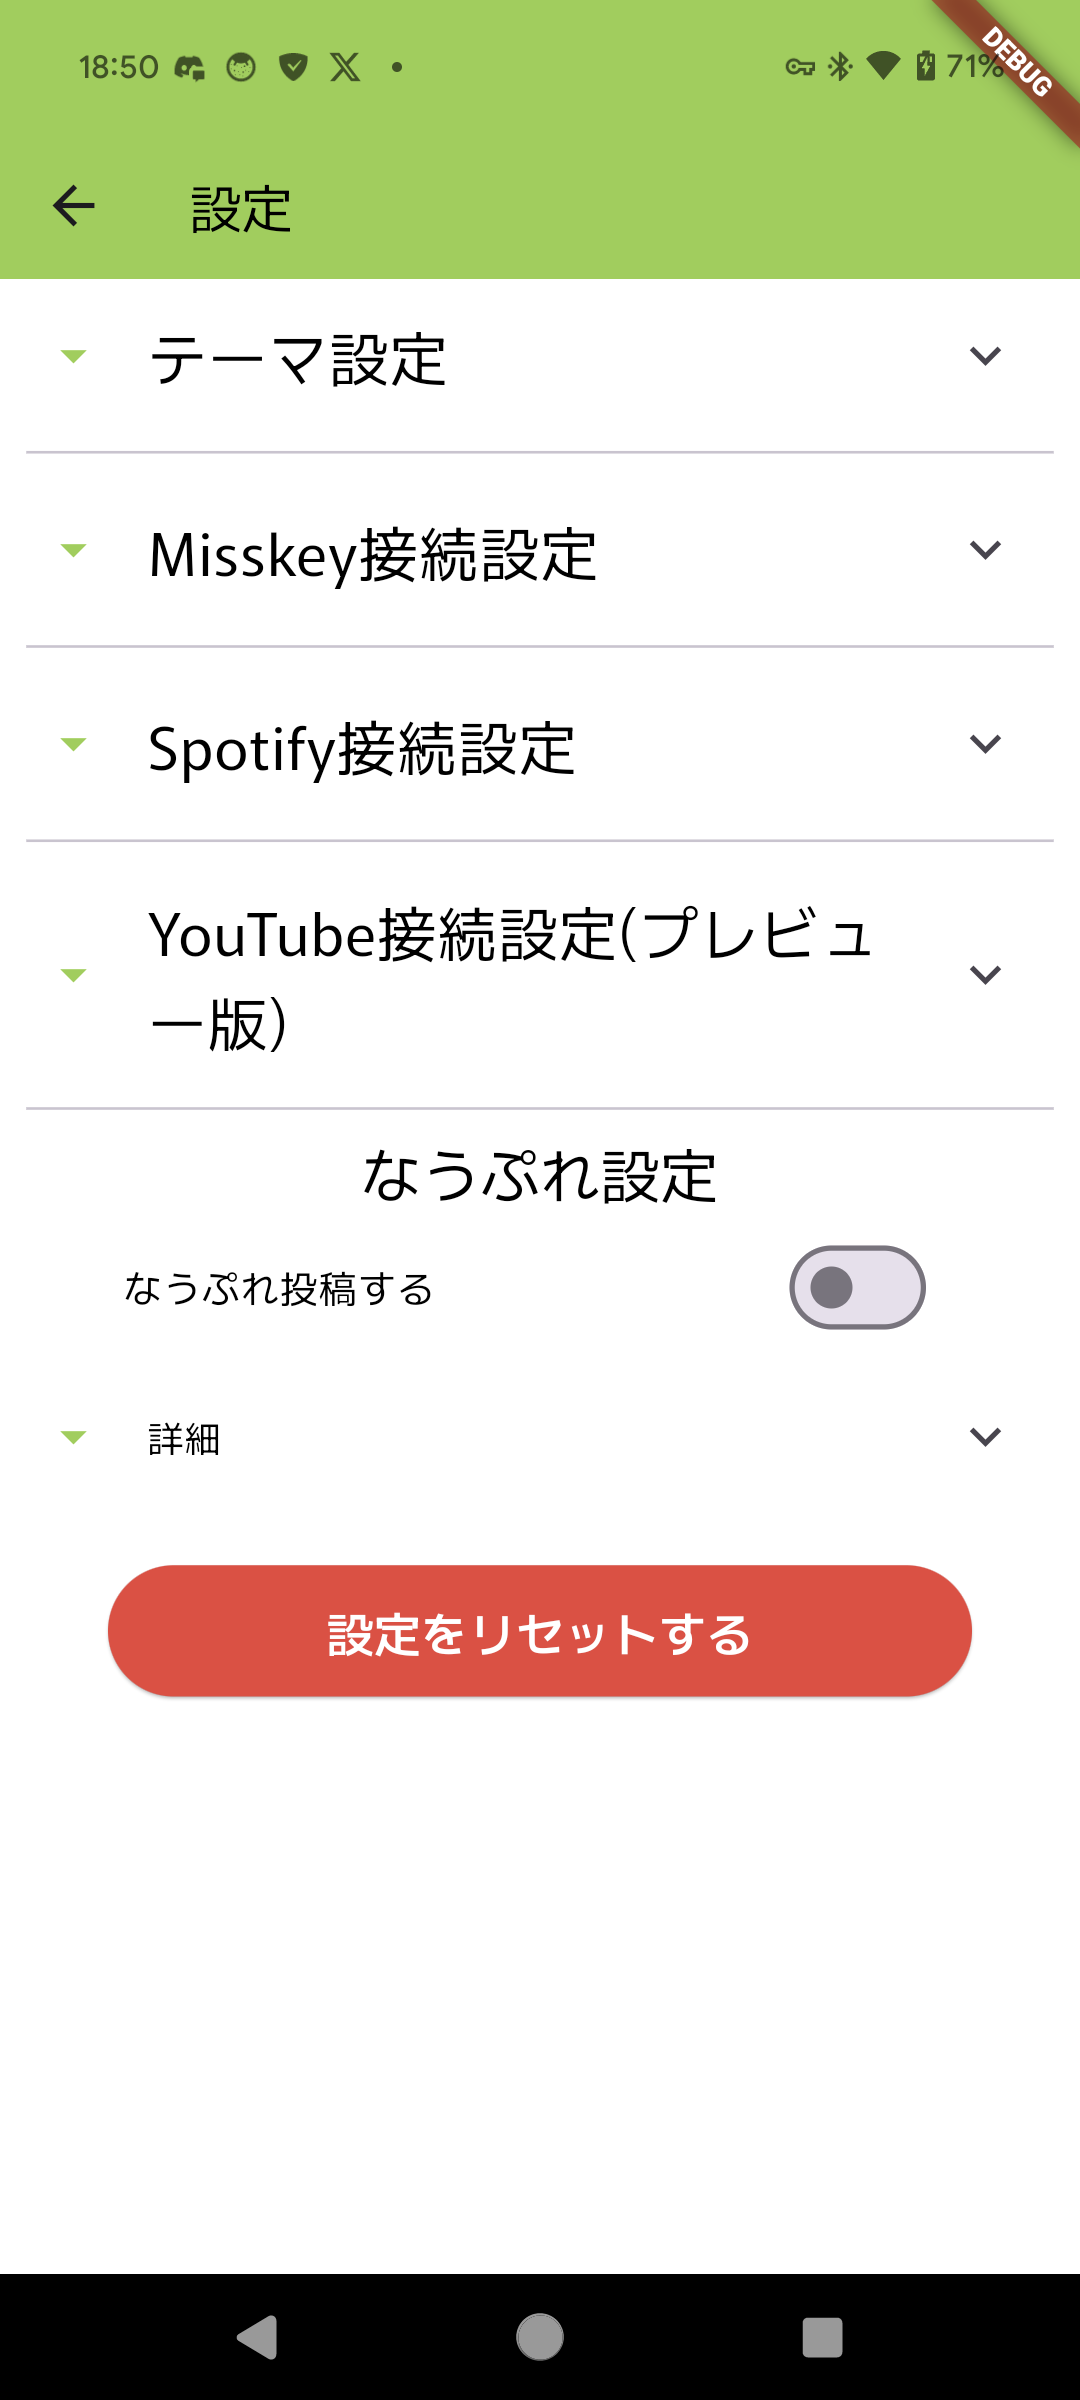
\includegraphics[width=5cm]{./pictures/lastfm11.png}
                        }
                        \caption{展開前}
                        \label{img:lastfm11}
                    \end{minipage}
                    \begin{minipage}[b]{0.45\linewidth}
                        \centering
                        \fbox{
                            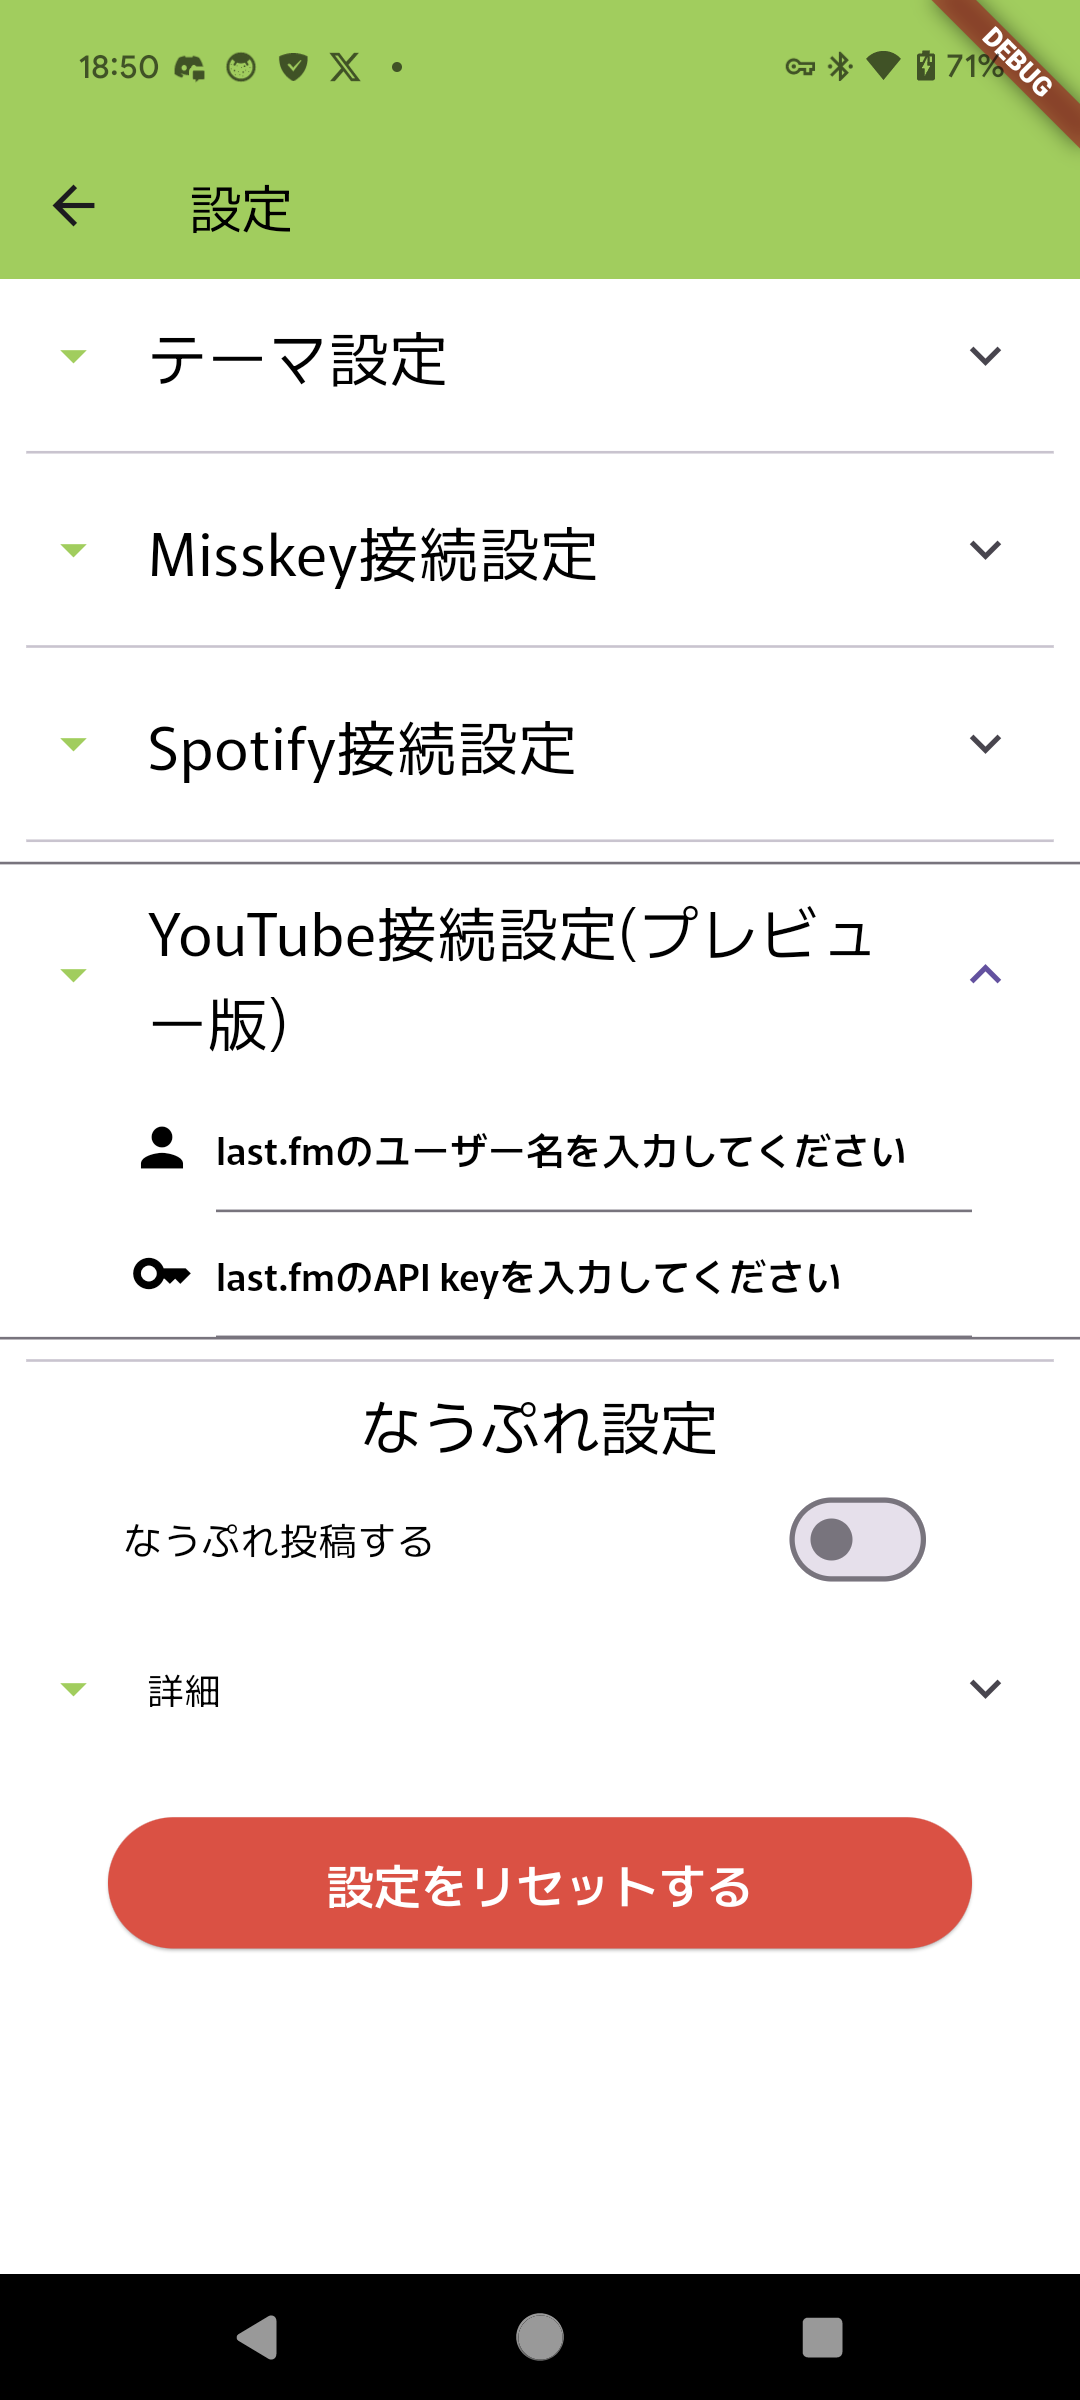
\includegraphics[width=5cm]{./pictures/lastfm12.png}
                        }
                        \caption{展開後}
                        \label{img:lastfm12}
                    \end{minipage}
                    \caption*{YouTube接続設定(プレビュー版)(\currentVersion)}
                \end{figure}

            \item \lastfm のユーザー名と、先ほど控えた\texttt{API key}を入力してください。
        \end{enumerate}